\chapter{Frameworks and IOC}
\section{Frameworks}

A \textbf{Software Framework}
is a collection of common code
providing generic functionality that can be selectively
overridden or specialized by user code providing
specific functionality.\\
An \textbf{Application Framework} is a software framework used to
implement the standard structure of an \textit{application} for
a specific development environment.

\labelitemize{Examples}{

   \begin{enumerate}
      \item General Software Frameworks
      \begin{enumerate}
         \item \texttt{.NET}
         \item \texttt{Android SDK}
         \item \texttt{Cocoa}
         \item \texttt{Eclipse}
      \end{enumerate}
      \item GUI Frameworks
      \begin{enumerate}
         \item \texttt{MFC}
         \item \texttt{Gnome}
         \item \texttt{Qt}
      \end{enumerate}
      \item Web Frameworks
      \begin{enumerate}
         \item \texttt{ASP.NET}
         \item \texttt{Rails}
         \item \texttt{GWT}
         \item \texttt{Spring}
         \item \texttt{Flask}
      \end{enumerate}
   \end{enumerate}
}

A framework embodies some \textit{abstract design}, with
more behavior built in.
In order to use it you need to insert your behavior into various places in the framework either by subclassing or by plugging in your own classes,
then 
the framework’s code, which handles the program's \textbf{control flow} (the "\texttt{main} execution"), then calls your code at these points.\\
This realizes a very general concept, emphasizing \textbf{inversion of
control} as opposed to libraries,
where the user's code calls the library one,
here is the code of the framework that calls the user's one.

\subsection{Component Frameworks}
\textbf{Componenent Frameworks} support development, deployment, composition
and execution of components designed according to a given
\textbf{Component Model}.
More specifically, they support \textbf{composition/connection} of components according to
the mechanisms provided by the \textit{Component Model},
allowing instances to be "plugged" into the
component framework itself,
and regulating their \textbf{interaction}.

\subsubsection{IDE and Frameworks}
\textbf{NetBeans} is both an \texttt{IDE} and supports the \texttt{JavaBeans} \textit{Component Framework}.\\
In general A framework can be supported by several \texttt{IDE}s
\note{
   e.g. \texttt{Spring} supported by \texttt{Spring Tool Suite} (based
   on \texttt{Eclipse}), \texttt{NetBeans}, \texttt{IntelliJ IDEA}, \texttt{Eclipse}, ...
} 
While an \texttt{IDE} can support several frameworks
\note{
   e.g \texttt{NetBeans} supports \texttt{JavaBeans}, \texttt{Spring}, \texttt{J2EE},
   \texttt{Maven}, \texttt{Hibernate}, \texttt{JavaServer Faces}, \texttt{Struts}, \texttt{Qt}, ...
} 

\subsection{Features}
Consist of \textbf{parts} that are found in many apps of that type
\begin{itemize}
   \item \textbf{Libraries} with APIs (classes with methods etc.)
   \item Ready-made extensible programs ("\textbf{engines}")
   \item Sometimes also \textbf{tools} (e.g. for development, configuration,
   content)
\end{itemize}
They also provide reusable abstractions of code wrapped in a well-defined API,
however recall that,unlike in libraries,
the overall program's \textbf{flow of control} is \textit{not} dictated by the caller, but by the \textit{framework}.
\nl

Frameworks usually support extensibility,
either by extending within the framework language {---} using, subclassing, overriding, implementing interfaces, registering event handlers, ...{---} or through plug-ins defined in a specific format.
 

\section{Inversion of Control}
\subsection{GUI}
In \textit{text-based interaction}, the order of interactions
and of invocations is decided by the the code,
while in the \textit{\textbf{GUI}-based interaction}, the \textit{GUI} loop decides
when to invoke the methods (listeners), based on the
order of events.

\begin{figure}[htbp]
   \centering
   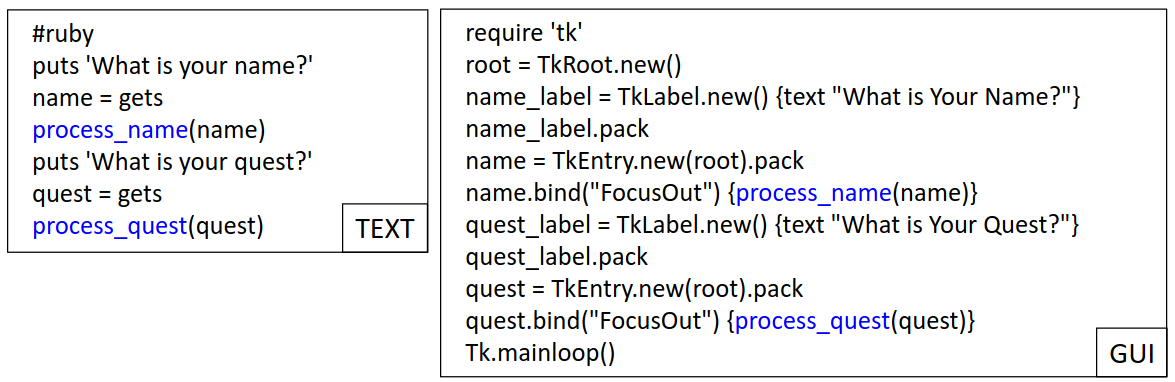
\includegraphics{images/ioc_textgui.png}
   \caption{Text vs GUI interaction}
   \label{fig:ioc_textgui}
\end{figure}

\begin{figure}[htbp]
   \centering
   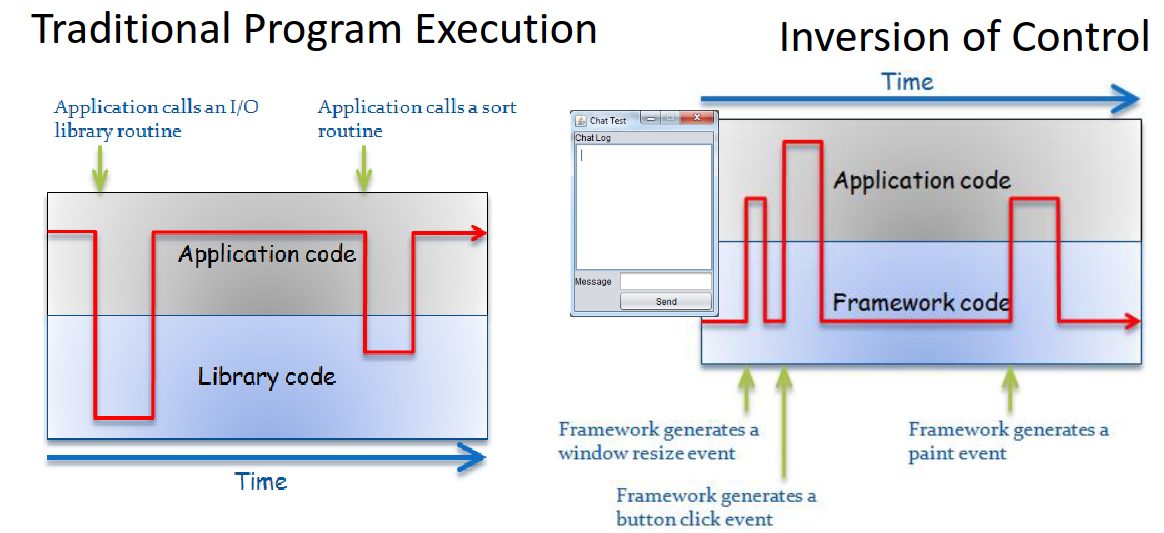
\includegraphics{images/ioc_fwvslib.png}
   \caption{IoC: Library vs Framework approach}
   \label{fig:ioc_fwvslib}
\end{figure}

\subsection{Containers}
Often Frameworks provide \textbf{containers} for deploying
\textit{components}:
a container may provide at \textit{runtime functionalities}
needed by the components to execute.

For examples \texttt{EJB} containers are responsible of the
persistent storage of data and of the availability of
\texttt{EJB}’s for all authorized clients.

\section{Loosely Coupled Systems}
Good \textit{OO Systems} should be organised as
network of interacting objects,
keeping in mind as a goal to have \textit{high \textbf{cohesion}}, \textit{low \textbf{coupling}}.\\
Low coupling has as key advantages
\begin{itemize}
   \item Extensibility
   \item Testability
   \item Reusability
\end{itemize}

\subsection{Dependecy Injection}
When discussing \textbf{IoC} in Frameworks, \textit{"Control"} does not refer only to control flow, but also control over \textit{dependencies},\textit{coupling}, \textit{configuration}.

We can make a few considerations on IoC with respect to dependencies:
\begin{itemize}
   \item 
   \item something outside a component handles:
   \begin{itemize}
      \item configuration (properties)
      \item wiring / dependencies (components)
   \end{itemize}
   \item component-oriented
   \item removes coupling
   \begin{itemize}
      \item coupling of configuration and dependencies to the point of use
      \item coupling of component to concrete dependent components
   \end{itemize}
   \item somewhat contrary to encapsulation
\end{itemize}

\section{Trade Monitor}
Let's discuss this  example to see how all of this comes into practice.
\begin{center}
   \textit{A trader wants that the system rejects trades when the exposure reaches a certain limit}
\end{center}

Thus the component (class) \texttt{TradeMonitor} provides
a method \texttt{TryTrade} (below) which checks the condition,
accessing \textit{current exposure} and \textit{exposure limit} from a \texttt{DAO} (\textit{Data Access Object}), a persistent storage.
\begin{lstlisting}
   public bool TryTrade(string symbol, int amount){
      int limit = limitDao.GetLimit(symbol);
      int exposure = limitDao.GetExposure(symbol);
      return (exposure + amount > limit) ? false : true;
      }
\end{lstlisting}
How can we limit dependencies among the two components?
\subsection{Interfaces - Refactoring 1}
Let's consider a possible refactoring, introducing \textbf{interface} and implementation separation,
which still has a static dependency on \texttt{DAO} :
\begin{figure}[htbp]
   \centering
   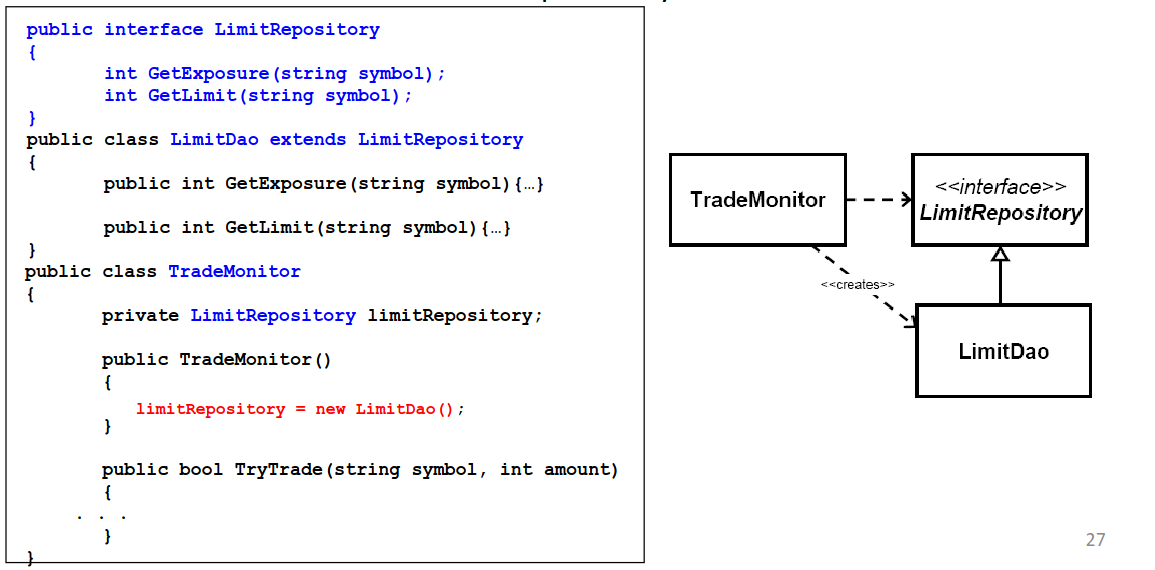
\includegraphics{images/trademonitor_ref1.png}
   \caption{Refactoring 1}
   \label{fig:trademonitor_ref1}
\end{figure}

\subsection{Factory - Refactoring 2}
Here we introduce a \textbf{factory} which resolves the previous problem, but \texttt{LimitDao} is still tightly coupled, but to \texttt{Factory}.

\begin{figure}[htbp]
   \centering
   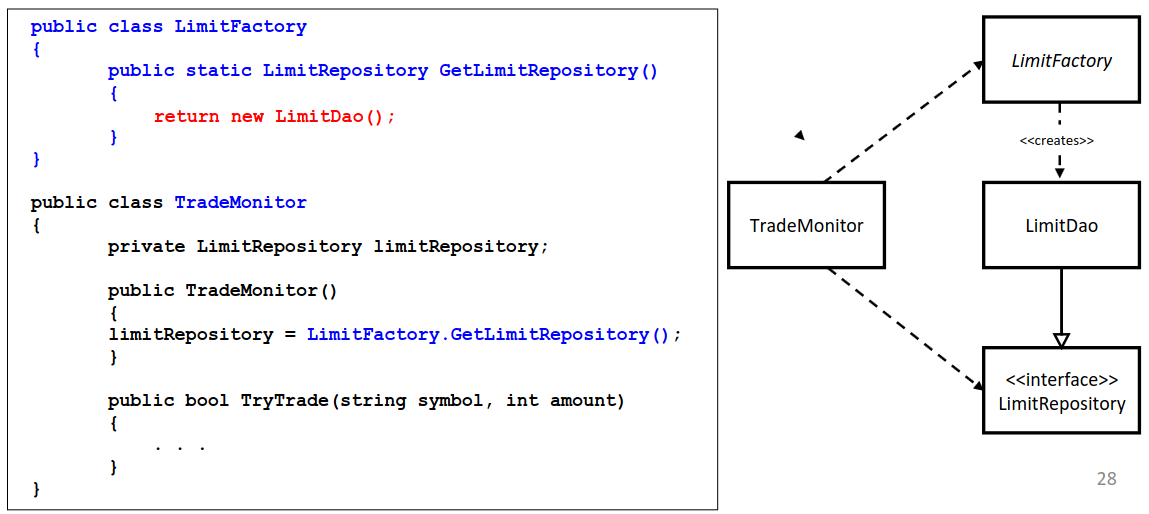
\includegraphics{images/trademonitor_ref2.png}
   \caption{Refactoring 2}
   \label{fig:trademonitor_ref2}
\end{figure}

\subsection{ServiceLocator - Refactoring 3}
Introduce a \texttt{ServiceLocator}. This object acts as a (static)
registry for the \texttt{LimitDao} you need,
giving us extensibility, testability, reusability.\\
However ote that an external \texttt{Assembler} sets up the registry.

\begin{figure}[htbp]
   \centering
   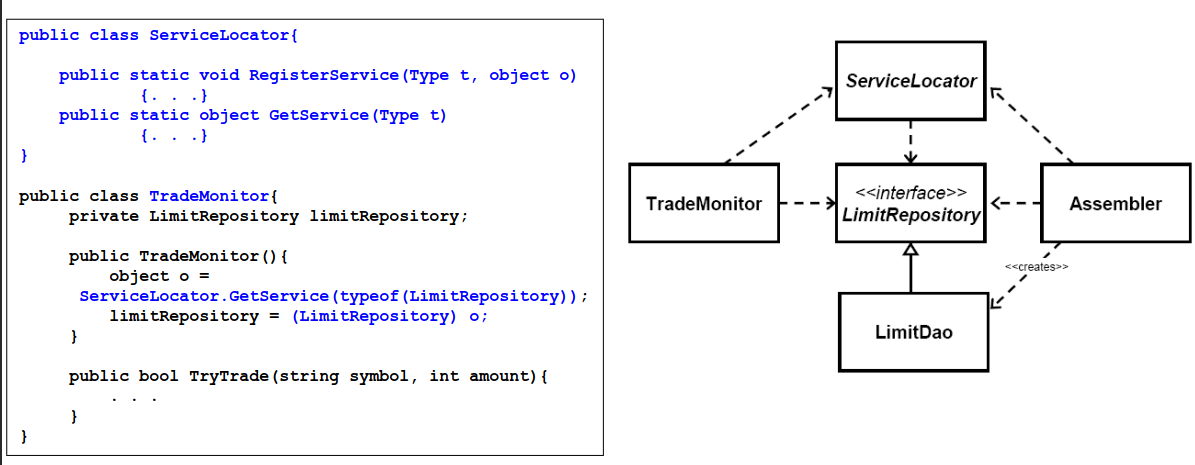
\includegraphics[width=0.7\columnwidth]{images/trademonitor_ref3.png}
   \caption{Refactoring 3}
   \label{fig:trademonitor_ref3}
\end{figure}

\labelitemize{
   \color{darkgreen}
   \textit{Pros}
}{
   \color{darkgreen}
   \begin{itemize}
      \item The Service Locator pattern succeeds in decoupling the TradeMonitor
      from the LimitDao
      \item Allows new components to be dynamically created and used by other
      components later
      \item It can be generalized in several ways, eg. to cover dynamic lookup
   \end{itemize}
}

\labelitemize{
   \color{darkred}
   \textit{Cons}
}{
   \color{darkred}
   \begin{itemize}
      \item Every component that needs a dependency must have a reference to the
      service locator
      \item All components need to be registered with the service locator
      \item If bound by name:
      \begin{itemize}
         \item Services can’t be type-checked
         \item Component has a dependency to the dependent component names
         \item if many components share an instance but later you want to specify different
      \end{itemize}
      instance for some, this becomes difficult
      \item If bound by type can only bind one instance of a type in a container
      \item Code needs to handle lookup problems
   \end{itemize}
}

\section{Dependency Injection}

\begin{figure}[htbp]
   \centering
   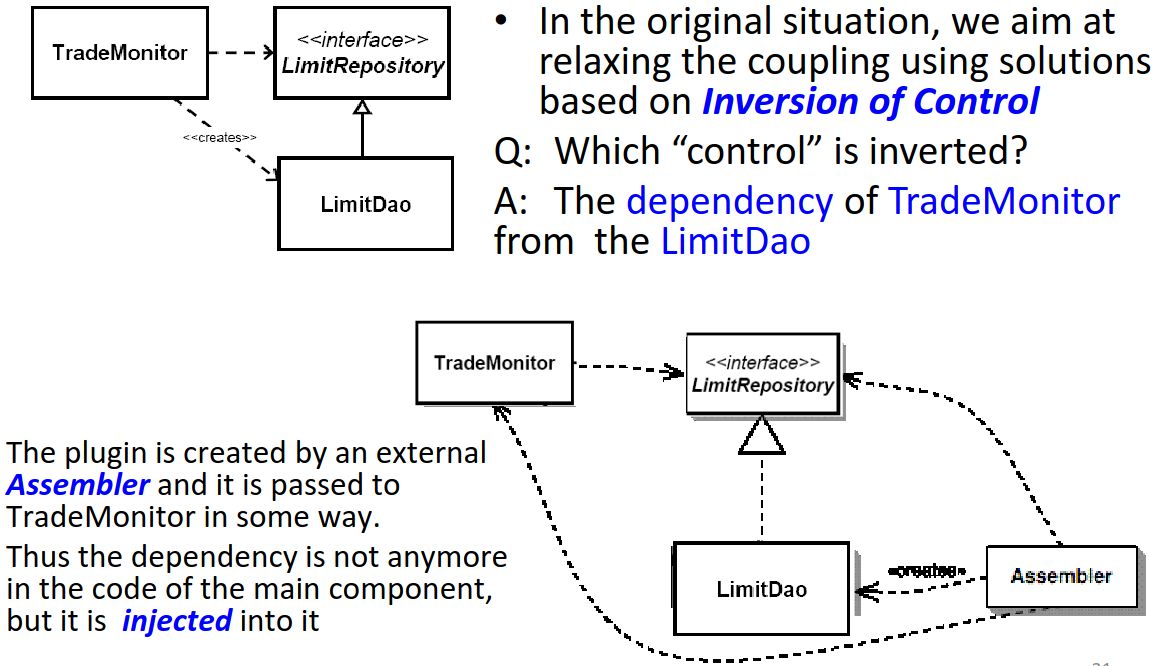
\includegraphics{images/dependency_inj.png}
   % \caption{}
   \label{fig:dependency_inj}
\end{figure}

\textbf{Dependency injection} allows avoiding \textit{hard-coded}
dependencies (strong coupling) and changing them, and allows selection among multiple implementations of a given dependency interface at run time.
It can be achieved through:
\begin{enumerate}
   \item Setter injection
   \item Constructor injection
   \item (Interface injection)
\end{enumerate}

Both \textbf{Service Locator} and \textbf{Dependency Injection} provide
the desired decoupling, but let's compare the two solutions: 
\begin{itemize}
   \item 
   With service locator there is no \textbf{IoC}, since the desired component is obtained
   after request by the \texttt{TradeMonitor} to the \texttt{Locator};
   this makes the application still depending on the locator.
   \item With dependency injection there is \textit{no explicit request}: the
   component appears in the application class.
\end{itemize}
Inversion of control a bit harder to understand, however,
it is easier to find dependencies of component if \textit{Dependency Injection} is used
\begin{center}
   \color{darkgray}
   Check \textit{constructors} and \textit{setters}\\vs\\Check \textit{all invocations} to
   \texttt{Locator} in the source code
\end{center}